考研主要涉及{\textbf{以下计算机性能指标:}}

\textbf{(1)吞吐量}

吞吐量指信息流入、处理和流出系统的速率。它取决于CPU能够多快地取指令,数据能够多快地从内存取出或存入,以及所得结果能够多快地从内存送到输出设备。这些决定因素中的任一步骤都与主存紧密相关,因此吞吐量主要取决于主存的存取周期。

\textbf{(2)响应时间}

响应时间指从提交作业到该作业得到CPU响应所经历的时间。响应时间越短,吞吐量越大。

\textbf{(3)主频}

主频是机器内部主时钟的频率,是衡量机器速度的重要参数,其常用单位为Hz、MHz等。如果主频为8MHz,则可以计算出时钟周期为: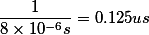
\includegraphics[width=1.55208in,height=0.36458in]{texmath/ee1758frac18times10-6s0125us}

即每秒有8M个时钟周期。

\textbf{(4)CPU周期}

CPU周期又称为机器周期,通常用从内存读取一条指令字的最短时间来定义。一个指令周期常由若干个CPU周期构成。

\textbf{(5)CPU时钟周期}

主频的倒数,是CPU中最小的时间单位。

\textbf{(6)CPI、MIPS和FLOPS(三者为衡量运算速度的指标)}

\textbf{CPI}:执行一条指令所需要的时钟周期数。

\textbf{MIPS}:每秒可执行百万条指令数,如某机器每秒可以执行800万条指令,则记作8MIPS。

\textbf{FLOPS}:每秒执行的浮点运算次数。

\textbf{MFLOPS}:每秒百万次浮点运算,与MIPS类似。

\textbf{GFLOPS}:每秒十亿次浮点运算。

\textbf{TFLOPS}:每秒万亿次浮点运算。

\textbf{PFLOPS}:每秒千万亿次浮点运算。

{补充:IPC:CPU的每一个时钟周期内所执行的指令数。}

\textbf{(7)CPU执行时间}

CPU执行时间指CPU对某特定程序的执行时间,例如,对于程序A和程序B,CPU执行程序A和程序B分别使用了2s和4s,则对于程序A和程序B而言,CPU执行时间分别是2s和4s。
